\section{Monaco Grand prix}

\subsection{Circuit Analysis}

\textbf{Circuit Name:} Circuit de Monaco (Monte Carlo, Monaco) \\
\textbf{Length:} 3.337 km - \textbf{Laps:} 78 - \textbf{Total Distance:} 260.286 km

\begin{figure}[H]
    \centering
    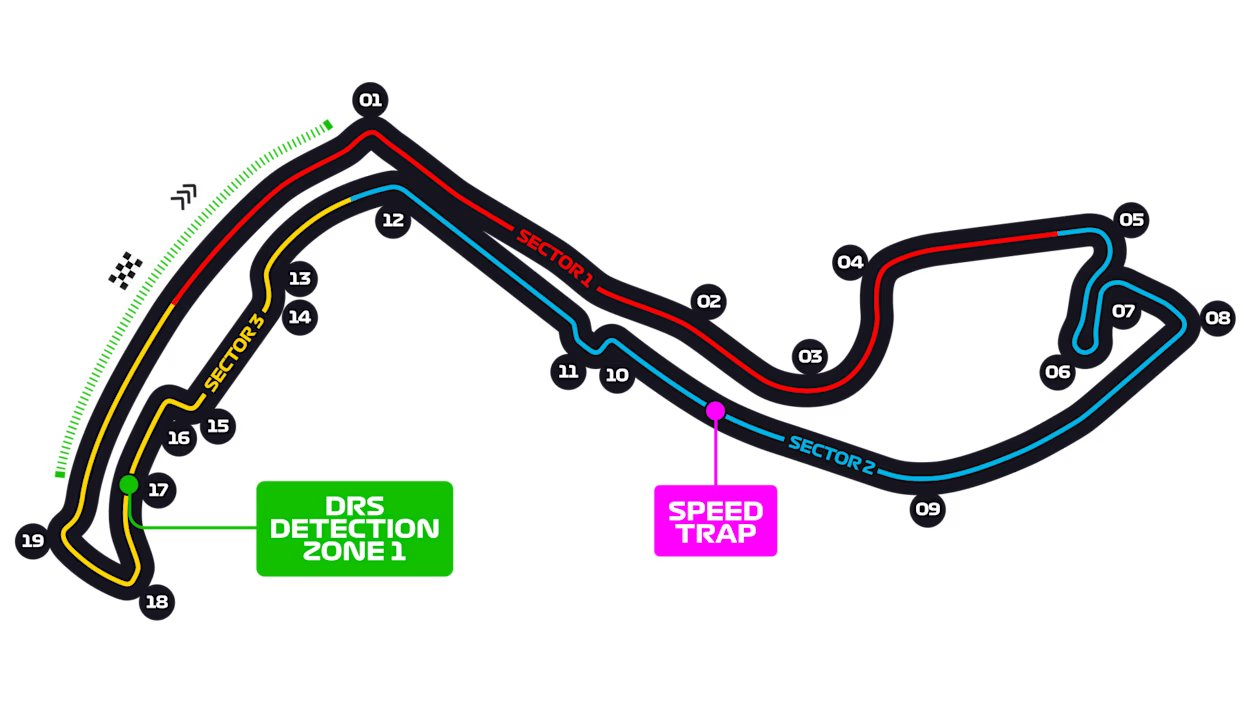
\includegraphics[width=0.75\linewidth]{images/8.Monaco_Circuit.jpg}
\end{figure}

\begin{itemize}
    \item \textbf{Lap Record} : 1:10.166 (2019, Lewis Hamilton – Mercedes).
    
    \item \textbf{Number of Corners \& Key Features} : 19 turns (11 right, 8 left) - Iconic layout through the streets of Monte Carlo, featuring tight hairpins (Grand Hotel Hairpin), fast tunnel section, and narrow barriers throughout.
    
    \item \textbf{Braking Zones \& Traction} : Major braking at Sainte Dévote (Turn 1), Mirabeau, and the Nouvelle Chicane. Traction critical out of the hairpin and Portier leading into the tunnel.
    
    \item \textbf{DRS \& Overtaking} : Single DRS zone along the main straight.\\
    Overtaking extremely limited, pit strategy and track position are decisive.
    
    \item \textbf{Tyre Degradation \& Strategy} : Tyre wear generally low, but graining can occur on softs.\\
    Most teams opted for one-stop, with pit timing more important than degradation.
    
    \item \textbf{Weather \& Environment} : Coastal location brings variable conditions, rain often change strategy. Narrow barriers punish even minor mistakes.
\end{itemize}

\textbf{Strategic Summary :}
Monaco rewards qualifying performance and flawless execution. Overtaking is almost impossible, so grid position and pit-stop timing are critical. Drivers must balance precision with risk around the unforgiving barriers.


\subsection{Race Analysis}

\textbf{Date:} 26 May 2024 — 15:00 local time 

\begin{itemize}
    \item \textbf{Qualifying Summary} : \textbf{Pole Position:} Charles Leclerc (Ferrari) – 1:10.270. \\
    Grid: Piastri 2nd, Sainz 3rd, Norris 4th.\\
    Verstappen only P6 after struggling in Q3.
    
    \item \textbf{Race Summary} : \textbf{Winner:} Charles Leclerc (Ferrari) - his first home victory.\\
    \textbf{Podium:} 1. Leclerc - 2. Piastri - 3. Sainz.\\
    \textbf{Notable incidents:} 
    - Perez and Magnussen collided on lap 1, both retired (red flag).\\
    - Ocon crashed into teammate Gasly at Portier, retired + 5-place grid penalty for Canada.
    
    \item \textbf{Strategies} : 
    - Red flag lap 1 allowed teams to switch tyres freely → most locked into a one-stop equivalent.\\ 
    - Leclerc controlled race on hard tyres, perfectly managing pace to keep Piastri behind. \\
    - Sainz strategically slowed Norris to avoid undercut threats from Russell. \\
    - Hamilton + Verstappen pitted late for fresh tyres to chase fastest lap → Hamilton succeeded on lap 63.
    
    \item \textbf{Performance Trends} : \textbf{Ferrari} delivered both one-lap speed and flawless race execution. Leclerc never relinquished the lead across 78 laps. \\
    \textbf{McLaren} continued strong form, Piastri competitive throughout, Norris closely behind. \\
    \textbf{Mercedes} solid but unspectacular — Russell P5, Hamilton P7 + fastest lap bonus. \\
    \textbf{Red Bull} struggled badly with setup and traction. Verstappen stuck in P6 all race, Pérez out on lap 1. \\
    \textbf{Tsunoda} consistent and secured more points for Racing Bulls. \\
    \textbf{Williams} scored their first points of the season with Albon P9. \\
    \textbf{Alpine} endured intra-team chaos. Gasly salvaged P10, Ocon retired lap 1. \\
    
    \item \textbf{Championship Impact} : \textbf{Drivers:} Verstappen 169 points, Leclerc 138, Norris 113 (+1).\\
    \textbf{Constructors:} Red Bull 276, Ferrari 252, McLaren 184, Mercedes 96.    
\end{itemize}

\textbf{Key Takeaway :}
Verstappen’s defensive driving under pressure secured victory. McLaren confirmed their rise with Norris pushing Verstappen to the limit. Ferrari solid but lacked enough speed to fight for the win at home.


\subsection{Link \& Takeaway}

\begin{itemize}
    \item Monaco once again proved the near impossibility of overtaking, qualifying dictated the race outcome. 
    \item The early red flag simplified strategies into an early one-stop, making overtaking virtually impossible.
    \item Ferrari capitalised perfectly on their one-lap advantage, securing both pace and control. 
    \item McLaren confirmed themselves as Ferrari’s closest challengers on high-downforce circuits. 
    \item Red Bull looked unusually vulnerable, with Verstappen unable to advance and Pérez eliminated lap 1. 
    \item Mercedes secured solid points but remain distant from Ferrari/McLaren pace. 
\end{itemize}